\documentclass[a4paper]{article}
\usepackage[utf8]{inputenc}
\usepackage[english]{babel}
\usepackage{amsmath}
\usepackage{graphicx}
\usepackage{xcolor}
\usepackage{hyperref}
\usepackage[margin=1in]{geometry}
\usepackage{capt-of}
\usepackage{blindtext}
\graphicspath{ {./images/} }
\definecolor{linkcolor}{HTML}{00F9DE}

\hypersetup{
  colorlinks=false,
  linkbordercolor=linkcolor,
  pdfborderstyle={/S/U/W 1}
}
\begin{document}
\section{The Proposed Method for Hand Gesture Recognition}

\subsection{The Overview of the Method}
The review of hand signal acknowledgment is depicted in Figure ~\ref{fig:The outline}. To begin with, the hand is distinguished utilizing the foundation deduction technique and the consequence of hand location is changed into a parallel picture. At that point, the fingers and palm are divided in order to encourage finger acknowledgment. Besides, the fingers are identified and perceived. Last, hand signals are perceived utilizing a straightforward guideline classifier.


\begin{figure}[h!]
 \begin{center}
  \includegraphics[scale=1.7]{fig1}
  \caption{The outline of the proposed strategy for hand signal acknowledgment.}
  \label{fig:The outline}
 \end{center}
\end{figure}




\subsection{Hand Detection}
The first pictures utilized for hand motion acknowledgment in the work are exhibited in figure ~\ref{fig:hand location}. These pictures are caught with an ordinary camera. These hand pictures are taken under a similar condition. The foundation of these pictures is indistinguishable. Thus, it is simple and compelling to recognize the hand locale from the first picture utilizing the foundation deduction technique. Nonetheless, sometimes, there are other moving articles remembered for the aftereffect of foundation deduction. The skin tone can be utilized to segregate the hand district from the other moving items. The shade of the skin is estimated with the HSV model. The HSV (tone, immersion, and worth) estimation of the skin tone is 315, 94, and 37, separately. The picture of the recognized hand is resized to 200x200 to make the motion acknowledgment invariant to the picture scale.


\begin{figure}[h!]
 \begin{center}
  \includegraphics[scale=1.7]{fig2}
  \caption{The system of hand location.}
  \label{fig:hand location}
 \end{center}
\end{figure}



\pagebreak

\subsection{Fingers and Palm Segmentation}
The yield of the hand discovery is a parallel picture wherein the white pixels are the individuals from the hand district, while the dark pixels have a place with the foundation. An illustration of the hand identification result is appeared in Figure ~\ref{fig:hand region}. At that point, the accompanying strategy is executed on the twofold hand picture to portion the fingers and palm.



\begin{figure}[h!]
 \begin{center}
  \includegraphics[scale=1.7]{fig3}
  \caption{The detected hand region.}
  \label{fig:hand region}
 \end{center}
\end{figure}



\subsubsection{Palm Point}
The palm point is characterized as the middle purpose of the palm. It is found by the strategy for distance change. Distance change likewise called distance map is a portrayal of a picture. Somewhere out there change the picture, every pixel records the distance between it and the closest limit pixel. An illustration of a distance change is exhibited in Figure ~\ref{fig:binary image}. Figure ~\ref{fig:binary image}(a) is a twofold picture and Figure ~\ref{fig:distance transform}(b) is the distance change picture. The square city distance is utilized to quantify the distances between the pixels and the closest limit pixels. As is appeared in the figure, the middle purpose of the twofold picture is with the biggest distance 4. In this way, somewhere out there change the picture (allude to Figure ~\ref{fig:The distance transform}) of the parallel hand picture, the pixel with the biggest distance is picked as the palm point. The discovered palm point is set apart with the purpose of the green tone in Figure ~\ref{fig:The palm point}.




\begin{figure}[h!]
 \begin{center}
\begin{minipage}[b]{0.4\textwidth}
  \includegraphics[scale=1.5]{fig4_a}
  \caption{(a) is a binary image}
  \label{fig:binary image}
 \end{minipage}
   \hfill
 \begin{minipage}[b]{0.4\textwidth}
  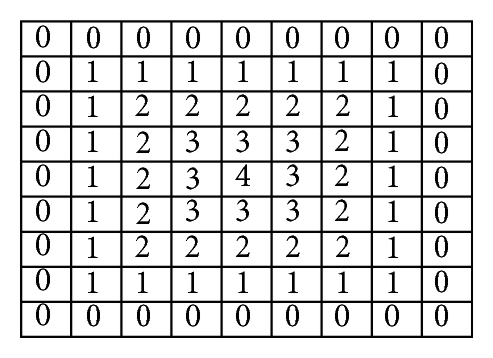
\includegraphics[scale=1.5]{fig4_b}
  \caption{(b) is the distance transform.}
  \label{fig:distance transform}
 \end{minipage}

 \end{center}
\end{figure}



\begin{figure}[h!]
 \begin{center}
  \includegraphics[scale=1.7]{fig4_c}
  \caption{The distance transform of the hand image.}
  \label{fig:The distance transform}
 \end{center}
\end{figure}


\begin{figure}[h!]
 \begin{center}
  \includegraphics[scale=1.7]{fig5}
  \caption{The palm point, wrist points, the wrist line, and the inner circle of the maximal radius.}
  \label{fig:The palm point}
 \end{center}
\end{figure}



\subsubsection{Inner Circle of the Maximal Radius}
At the point when the palm point is discovered, it can draw a hover with the palm point as the middle point inside the palm. The circle is known as the inward circle since it is incorporated inside the palm. The span of the circle bit by bit increments until it arrives at the edge of the palm. That is the sweep of the hover stops to increment when the dark pixels are remembered for the circle. The circle is the internal hover of the maximal range which is drawn as the hover with the red tone in Figure ~\ref{fig:The palm point}.

\subsubsection{Wrist Points and Palm Mask}
At the point when the span of the maximal internal circle is obtained, a bigger circle the sweep of which is 1.2 occasions that of the maximal inward circle is delivered. The circle is drawn as the blue shading circle in Figure ~\ref{fig:The palm point}. At that point, a few focuses (X,Y) are examined consistently along the circle. That is,

\begin{equation}
{arg_{P_{i},P_{i+1}}max(P_{i},P_{i+1})},\textrm{  } {P_{i},P_{i+1}} \textrm{  } \epsilon \textrm{  } S,
\end{equation}
\\
where $S$ is the set of palm mask points and $dist(*,*)$ is the distance between two points. Please refer to Figure 5 for the wrist points and wrist line.
\\
For each examined point on the circle, its closest limit point is found and lined to it. The limit point is decided in a basic manner. In the event that the 8 neighbors of a pixel comprise of white and dark pixels, it is named as a limit point. The entirety of the closest limit focuses discovered are connected to yield the palm veil that can be utilized to section fingers and the palm. The strategy for looking through the palm cover is depicted in Algorithm 1. The palm cover of the hand picture of Figure ~\ref{fig:hand region} is shown in Figure ~\ref{fig:The palm mask.}. A bigger hover rather than the maximal inward circle is utilized in order to yield a more exact palm veil for the accompanying division.


\begin{figure}[h!]
 \begin{center}
  \includegraphics[scale=1.7]{fig6}
  \caption{The palm mask.}
  \label{fig:The palm mask.}
 \end{center}
\end{figure}



\subsubsection{Hand Rotation:} 
When the palm point and wrist point are acquired, it can yield a bolt pointing from the palm to highlight the central purpose of the wrist line at the lower part of the hand. At that point, the bolt is acclimated to the heading of the north. The hand picture turns simultaneously to make the hand motion invariant to the pivot. In the interim, the parts underneath the waistline in the pivoted picture are sliced to deliver an exact hand picture that does not encase the arm's piece. Figure ~\ref{fig:The rotated and cut hand image.} is a turned and cut hand picture.

\begin{figure}[h!]
\begin{center}
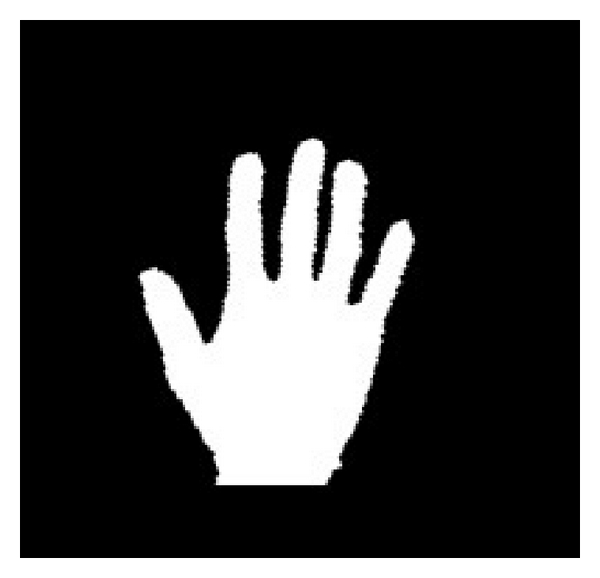
\includegraphics[scale=1.5]{Fig7}
\captionof{figure}{The rotated and cut hand image.}
 \label{fig:The rotated and cut hand image.}
\end{center}
\end{figure}

\subsubsection{Fingers and Palm Segmentation}
With the assistance of the palm veil, fingers and the palm can be sectioned without any problem. The hand covered by the palm veil is the palm, while different pieces of the hand are fingers. A division consequence of fingers and the palm appears in Figure ~\ref{fig:The segmented fingers.}.

\begin{figure}[h!]
\begin{center}
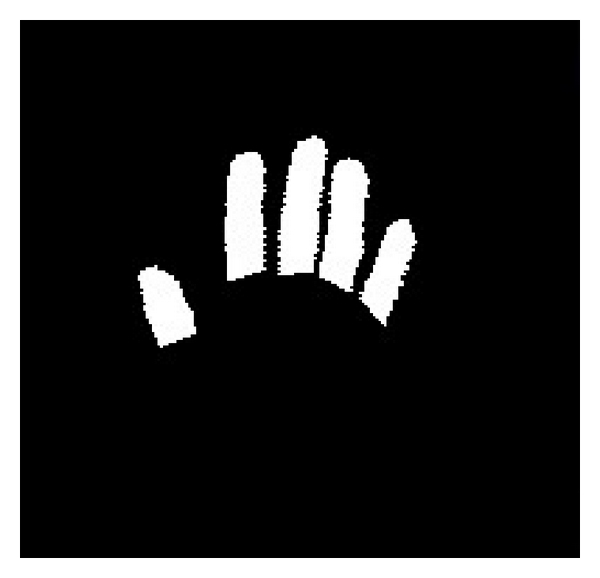
\includegraphics[scale=1.5]{Fig8}
\captionof{figure}{The segmented fingers.}
\label{fig:The segmented fingers.}
\end{center}
\end{figure}

\subsubsection{Fingers Recognition}
In the fingers' division picture, the naming calculation is applied to check the fingers' locales. As the consequence of the naming strategy, the identified districts where the number of pixels is too little are viewed as loud and disposed. Just the locales of enough sizes are viewed as fingers and remain. For each remained locale, that is, a finger, the little jumping box is found to encase the finger. A little bouncing box is signified as a red square shape in Figure ~\ref{fig:The minimal bounding box.}. At that point, the little jumping box's focal point is utilized to speak to the finger's middle purpose.


\begin{figure}[h!]
\begin{center}
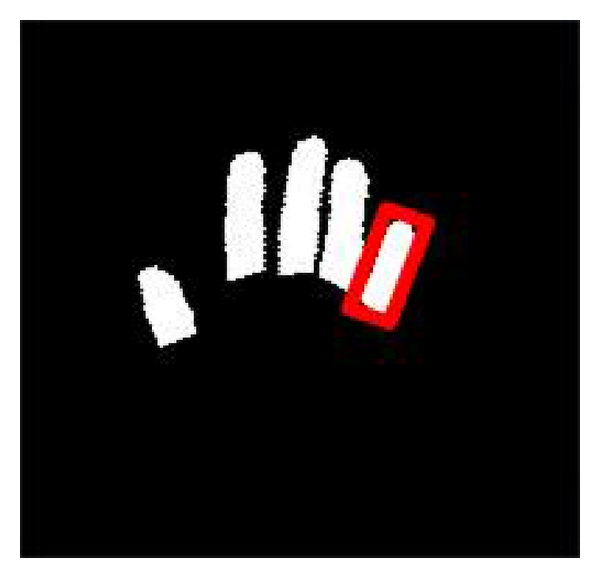
\includegraphics[scale=1.5]{Fig9}
\captionof{figure}{The minimal bounding box.}
\label{fig:The minimal bounding box.}
\end{center}
\end{figure}

\subsubsection{Thumb Detection and Recognition:}
The focuses of the fingers are lined to the palm point. At that point, the degrees between these lines and the wrist line are figured. If there is a degree more modest than, it implies that the thumb shows up in the hand picture. The relating focus is the middle purpose of the thumb. The identified thumb is set apart from number 1. If all the degrees are more significant than, the thumb does not exist in the picture.


\subsubsection{Detection and Recognition of Other Fingers:}
The palm line equals the wrist line. The palm line is looked at in a manner: start from the column of the wrist line. For each line, a line resembling the wrist line crosses the hand. On the off chance that there is just one associated set of white pixels in the line's crossing point and the hand, the line moves upward. Once there are more than one associated set of white pixels in the crossing point of the line and the hand, the line is viewed as a palm line competitor. On account of the thumb not distinguished, the line crossing the hand with more than one associated set of white pixels in their convergence is picked as the palm line. On account of the thumb existing, the line keeps moving upward with the edge purposes of the palm rather than the thumb as the beginning stage of the line. Presently, since the thumb is removed, there is just one associated set of pixels in the line's crossing point and the hand. When the associated set of white pixels goes to 2 once more, the palm line is found. The hunt of the palm line has appeared in Figure ~\ref{fig:The palm line.}.

\begin{figure}[h!]
\begin{center}
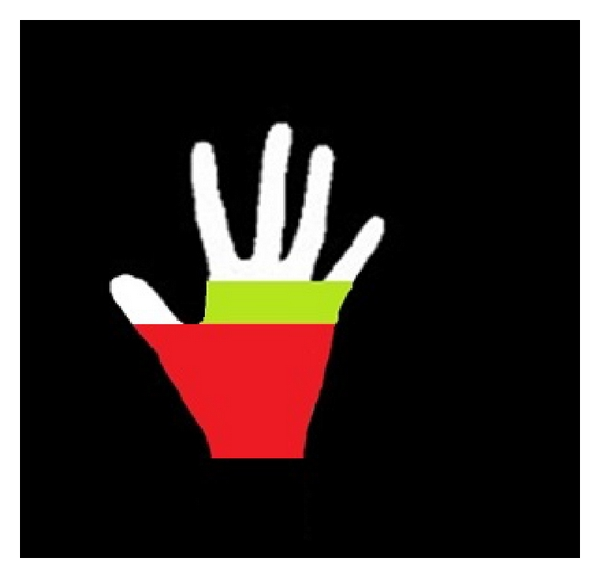
\includegraphics[scale=1.4]{Fig10}
\captionof{figure}{The palm line.}
\label{fig:The palm line.}
\end{center}
\end{figure}

After the palm line is acquired, it is partitioned into four sections. As per the even arrangement of the middle purpose of a finger, it falls into specific parts. If the finger falls into the initial segment, it is the pointer. If the finger has a place with the next part, it is the center finger. The third part compares to the ring finger. The fourth part is the little finger. The consequence of finger acknowledgment of Figure ~\ref{fig:hand region} is shown in Figure ~\ref{fig:The recognition of the fingers.}. The yellow line is the palm line in the figure, and the red line equals the wrist line.

\begin{figure}[h!]
\begin{center}
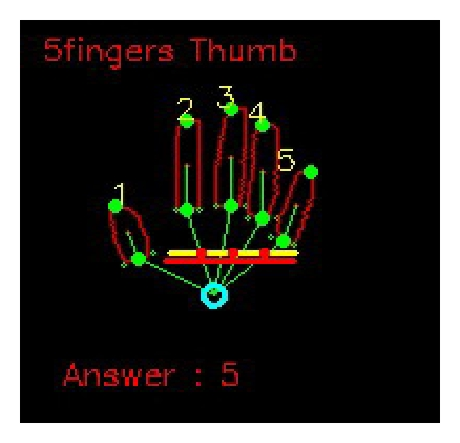
\includegraphics[scale=1.5]{Fig11}
\captionof{figure}{The recognition of the fingers.}
\label{fig:The recognition of the fingers.}
\end{center}
\end{figure}

At times, at least two fingers stay intently, and there is no stretch among the fingers. A case of the case is alluded to in Figure \ref{fig:The recognition of the fingers.}. The little bounding box's width is utilized as a segregation record to separate the case from a solitary finger. The distinguished district is a solitary finger on the off chance that the little bounding box's width is equivalent to a standard worth. On the off chance that the little bounding box's width is a few times the typical worth, the distinguished area relates to a few fingers that stay together intently. For the strength of finger acknowledgment, the separations and points between fingers are additionally considered to segregate various signals.


\subsubsection{Recognition of Hand Gestures}
When the fingers are distinguished and perceived, the hand signal can be perceived utilizing a straightforward standard classifier. In the standard classifier, the hand signal is anticipated by the number and substance of fingers recognized. The substance of the fingers implies what fingers are recognized. The standard of the classifier is extraordinarily compelling and productive. For instance, if three fingers, that is, the center finger, the ring finger, and the little finger, are distinguished, the hand signal is named mark 3 (allude to Figure 12 for the hand motions' names).

\begin{center}
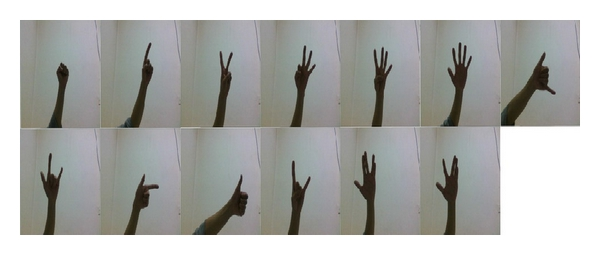
\includegraphics[scale=2.8]{Fig12}
\captionof{figure}{The image set of hand gestures used in the experiments. From left to right and then from top to bottom; these gestures are labeled as 0, 1, 2, 3, 4, 5, 6, 7, 8, 9, S1, S2, and S3.}
\end{center}


\section{Experimental Results} 
Data Set:
\linebreak
In the tests, two informational indexes of hand signals are utilized to assess the proposed strategy's presence. Informational index 1 is a picture assortment of thirteen signals. For each signal, 100 pictures are caught. In this way, there is a sum of 1300 pictures for hand signal acknowledgment. All the signal pictures have a place with three females and four guys. The size of one signal picture is 640x480.
\\
Another informational index is gathered from 10 subjects, and it contains ten signals for numbers 0 to 9. In this way, there is a sum of 10x10x10 cases. The informational index caught in jumbled foundations is an excellent test for hand motion acknowledgment. Plus, for each motion, the subject stances with varieties close by direction, scale, verbalization. We contrast our strategy and FEMD on the informational collection. 
\\

\subsection{Performance Evaluation on Data Set:1}

\subsubsection{Classification Accuracy}
To quantify the proposed hand signal acknowledgment strategy exhibition, the characterization exactness is assessed in the investigations. In the preparation stage, the standards separating the thirteen signals are created. At that point, the standard classifier utilizes the principles to foresee the personality of the testing picture. In Figures 3, 4, 5, 6, and 7, the five motions' acknowledgment is illustrated. There are six subfigures in each figure: the pictures indicating the parallel hand picture, the palm print, the wrist line, the aligned hand picture, the palm veil, the distinguished fingers, and finger and signal acknowledgment separately. In the subfigure of finger and motion acknowledgment, the name of the motion is anticipated. The anticipated mark is appeared behind "Answer."




\begin{center}

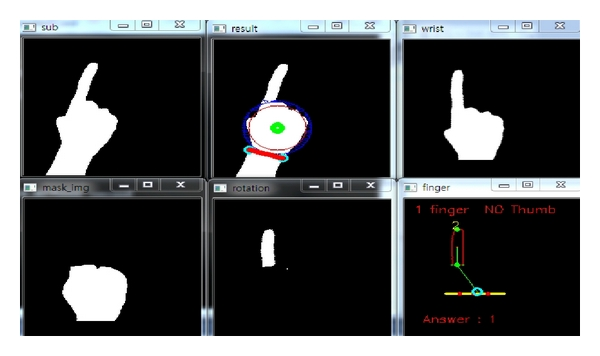
\includegraphics[scale=1.3]{Fig13}
\captionof{figure}{The recognition of the hand gesture 1.}

\vspace{1cm}

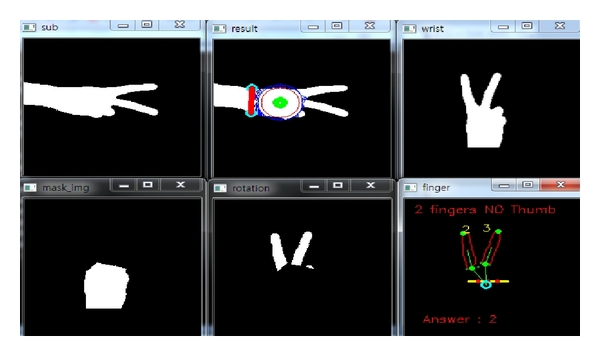
\includegraphics[scale=1.3]{Fig14}
\captionof{figure}{The recognition of the hand gesture 2.}

\vspace{1cm}

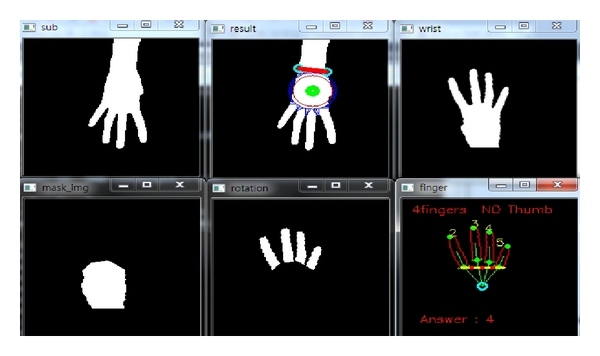
\includegraphics[scale=1.3]{Fig15}
\captionof{figure}{The recognition of the hand gesture 3.}

\vspace{1cm}

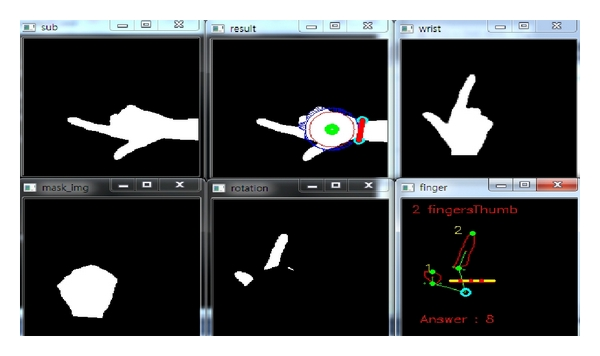
\includegraphics[scale=1.3]{Fig16}
\captionof{figure}{The recognition of the hand gesture 4.}

\vspace{1cm}

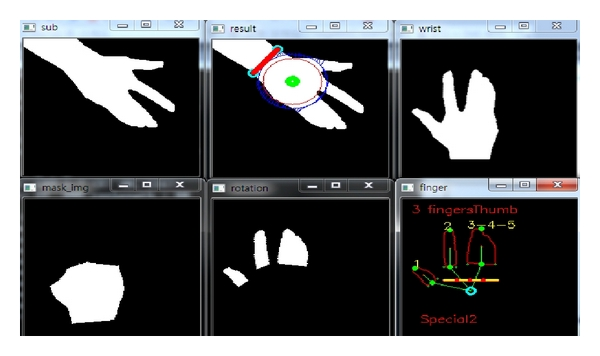
\includegraphics[scale=1.3]{Fig17}
\captionof{figure}{The recognition of the hand gesture 5.}
\end{center}


The arrangement aftereffects the absolute of 1300 pictures is summed up with a disarray lattice in Table 1. In the disarray network, the main section and the last line are the marks of the signals. Different passages of the lattice record the quantities of the signal pictures anticipated as the comparing marks. For instance, for the primary line, the numbers 99 and 1 are in the sections relating to the marks 1 and 3, separately. It implies that there are 99 and 1 pictures anticipated as the marks 1 and 3 in the 100 testing pictures of the motion 1. Along these lines, for the testing pictures of signal 1, the order precision is 99\%. As appeared in the disarray lattice, the proposed strategy performs well and acquires high arrangement precision. The all-out grouping exactness of the 1300 testing picture is 96.69\%. In the disarray framework, the offers of S2 and S3 are misclassified as 5. The explanation is portrayed as follows: for specific offers of S2 and S3, the fingers do not remain shut. That is, there is an opening between two fingers. In this way, in these cases, the offers of S2 and S3 are misclassified as 5.

\begin{center}
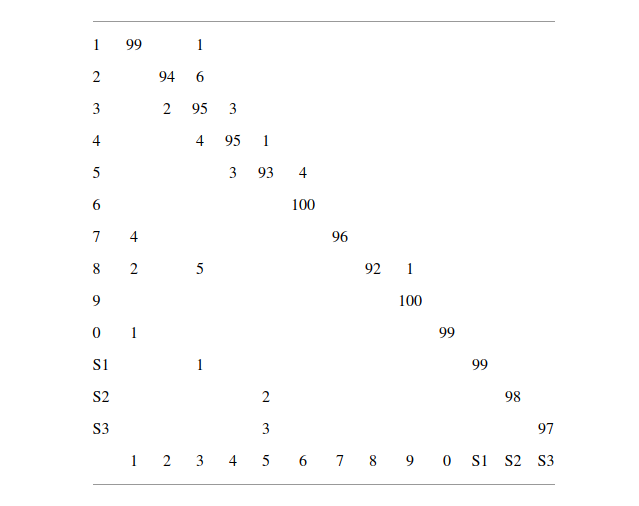
\includegraphics[scale=0.26]{Table1}
\captionof{table}{The confusion matrix of hand gesture recognition on data set 1.}
\end{center}


\subsubsection{Time Cost:}
The time cost for perceiving the motions is accounted for in Table 2. In the table, the unit of the time cost is second. An incentive in the subsequent line is the averaging runtime of 100 pictures of one signal. For the complete 1300 pictures, the average time cost to perceive hand motions is 0.024 seconds. The analyses are run on the PC Intel i7-2630 2.00 GHz CPU and 4 GB RAM. The proposed strategy is advantageous and can meet the prerequisite of ongoing applications.

\begin{center}
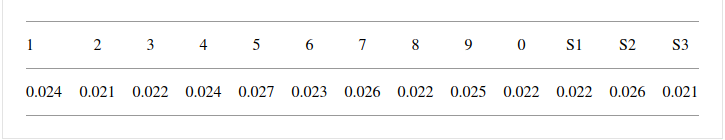
\includegraphics[scale=0.3]{Table2}
\captionof{table}{The runtime of hand gesture recognition.}
\end{center}



\subsection{Performance Comparison on Data Set 2:}
The correlation of the proposed strategy and a condition of-workmanship technique FEMD is performed on informational index 2. The order results are likewise summed up with the disarray grids. The portrayal of the disarray networks is like that in Table 1. The disarray framework of our technique has appeared in Table 3. The disarray lattice of FEMD is shown in Table 4. The averaging precision of the proposed strategy is 96.6\%. The averaging exactness of FEMD is 93.2\%. The examination results on informational collection 2 show that our strategy beats FEMD. The averaging season of our technique spent on perceiving a hand signal is 0.0202 seconds
\cite{DUMMY:1}
\begin{center}
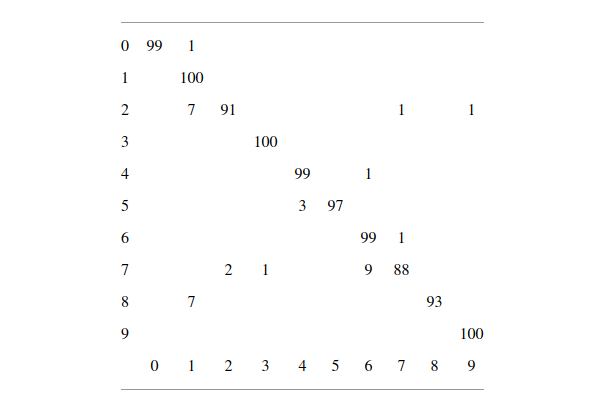
\includegraphics[scale=0.3]{Table3}
\captionof{table}{The confusion matrix of our method on data set 2.}
\end{center}


\begin{center}
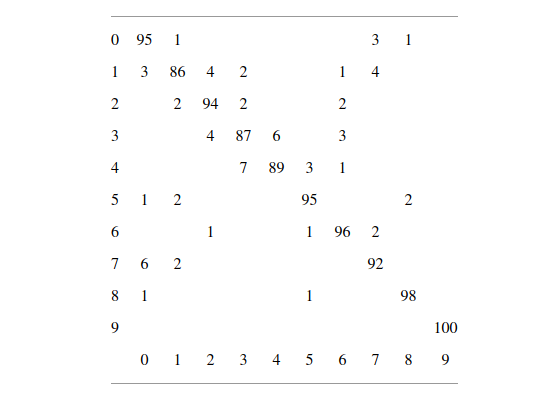
\includegraphics[scale=0.3]{Table4}
\captionof{table}{The confusion matrix of FEMD on data set 2.}
\end{center}

\bibliography{biblo} 
\bibliographystyle{ieeetr}
\end{document}
